\documentclass[aspectratio=169,10pt]{beamer}
\usetheme{Madrid}\usecolortheme{default}
\usepackage{amsmath,amssymb,graphicx,booktabs}
\definecolor{groupblue}{RGB}{53,48,173}
\setbeamercolor{structure}{fg=groupblue}
\setbeamercolor{title}{bg=groupblue,fg=white}
\setbeamercolor{frametitle}{bg=groupblue,fg=white}
\setbeamercolor{block title}{bg=red!45!black,fg=white}
\setbeamercolor{block body}{bg=black!4,fg=black}
\setbeamerfont{block title}{size=\small}
\setbeamerfont{block body}{size=\footnotesize}
\setbeamertemplate{navigation symbols}{}
\setbeamersize{text margin left=8mm,text margin right=8mm}
\title[Periodic advection]{Numerical Dissipation, Dispersion and TVD\\for the Periodic Advection Equation}
\subtitle{Accuracy, fidelity and measured computational cost}
\author[Group C]{Group C\\[2mm]\small Chuqiao Tang (2360692), Jinyu Ma (2363433)\\
Muqing Xu (2362900), Shuoran Fu (2362626)\\
Taiqi Zhang (2363684), Yujia Ding (2362094)}
\institute[MTH321 Project 3]{MTH321 Numerical PDEs --- Project 3}
\date[November 2026]{November 2026}
\begin{document}
\begin{frame}[plain]
\titlepage
\end{frame}
\begin{frame}{Research question and controlled model}
\begin{block}{Research question}How do schemes balance accuracy, dissipation, dispersive oscillations and cost for smooth and discontinuous data?\end{block}\[u_t+u_x=0,\quad x\in[0,1),\qquad u(x,t)=u_0((x-t)\bmod1).\]\begin{itemize}\item Dimensionless units and periodic indices\item Point values $x_j=j/N$, no duplicate endpoint\item Sine, smooth periodic packet and half-open square\end{itemize}
\end{frame}
\begin{frame}{Baseline updates from the PDE}
\textbf{Upwind:} forward time and upstream space\[U_j^{n+1}=U_j^n-C(U_j^n-U_{j-1}^n).\]\textbf{Lax--Wendroff:} Taylor in time, $u_{tt}=u_{xx}$\[U_j^{n+1}=U_j^n-\tfrac C2(U_{j+1}^n-U_{j-1}^n)+\tfrac{C^2}2(U_{j+1}^n-2U_j^n+U_{j-1}^n).\]\small Every index wraps modulo $N$. Both updates conserve discrete mass.
\end{frame}
\begin{frame}{Diffusion and dispersion have different mechanisms}
\[u_t+u_x\approx\tfrac h2(1-C)u_{xx}\quad\text{(upwind)},\]\[u_t+u_x\approx-\tfrac{h^2}6(1-C^2)u_{xxx}\quad\text{(LW)}.\]\begin{itemize}\item Upwind loses amplitude and spreads fronts\item LW changes phase and permits ripples at jumps\item LW right-neighbour weight $(C^2-C)/2<0$ for $0<C<1$\end{itemize}
\end{frame}
\begin{frame}{MC limits the antidiffusive correction}
\[F_{j+1/2}=U_j+\tfrac12(1-C)s_j,\qquad U_j^{n+1}=U_j-C(F_{j+1/2}-F_{j-1/2}),\]\[s_j=\phi(r_j)(U_{j+1}-U_j),\quad r_j=\frac{U_j-U_{j-1}}{U_{j+1}-U_j},\]\[\phi_{\rm MC}(r)=\max(0,\min(2r,(1+r)/2,2)).\]\small Signed-minimum implementation avoids division. Zero or opposite-sign slopes give zero correction. Minmod is a sensitivity comparison.
\end{frame}
\begin{frame}{TVD proof applies to this complete update}
\[\operatorname{TV}(U)=\sum_j|U_j-U_{j-1}|.\]\[U_j^{n+1}=U_j-A_j(U_j-U_{j-1}),\qquad C^2\le A_j\le2C-C^2\le1.\]\[d_j^{n+1}=(1-A_j)d_j+A_{j-1}d_{j-1}.\]\begin{itemize}\item Triangle inequality and periodic summation prove TVD\item Assumptions: scalar, constant speed, uniform grid, $0\le C\le1$\item Limiting near extrema can reduce local accuracy\end{itemize}
\end{frame}
\begin{frame}{Linear Fourier factors and the CFL boundary}
\[G_{\rm up}=1-C+Ce^{-i\xi},\quad |G_{\rm up}|^2=1-4C(1-C)\sin^2(\xi/2),\]\[G_{\rm LW}=1-iC\sin\xi-2C^2\sin^2(\xi/2),\]\[|G_{\rm LW}|^2=1-4C^2(1-C^2)\sin^4(\xi/2).\]\small Circulant periodic matrices make Fourier analysis applicable. All admissible modes contract for $|C|\le1$ with the sign-corrected upwind stencil.
\end{frame}
\begin{frame}{Verification includes a hand-computable seam test}
\[U=[0,1,2,0],\quad C=\tfrac12.\]\begin{align*}\text{Upwind}:&\ [0,1/2,3/2,1],\\\text{LW}:&\ [-1/8,1/2,15/8,3/4],\\\text{MC}:&\ [0,3/8,13/8,1].\end{align*}\begin{itemize}\item 77 automated tests pass\item Scalar loops independently reproduce vector updates\item Two incorrect initial expected arrays were corrected and logged\end{itemize}
\end{frame}
\begin{frame}{Separated error needs a declared reference}
\[B_{\rm LW}(\Delta t)=I+\Delta t A_0+\tfrac12\Delta t^2D_2,\qquad D_2\ne A_0^2.\]\begin{itemize}\item Space: exact-in-time limiting operator versus exact PDE\item Time: fixed $N=100$ versus the same-grid limit\item Classical LW is generally first order relative to this limit\item MC reference uses tolerance-refined limited-flux ODE integration\end{itemize}
\end{frame}
\begin{frame}{Measured refinement rates}
\centering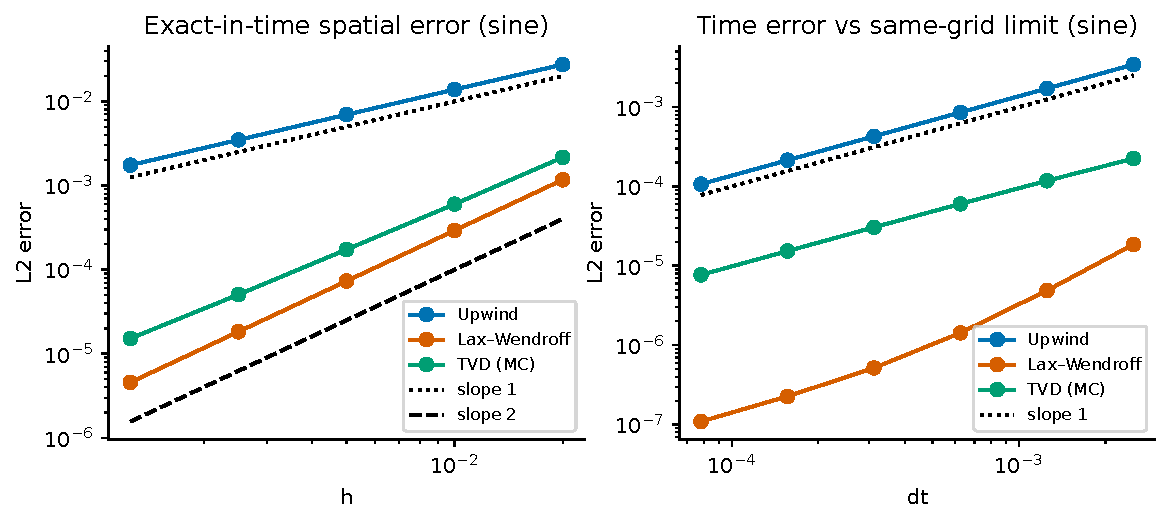
\includegraphics[width=.78\linewidth]{../results/figures/separated_convergence.pdf}\par\vspace{1mm}\begin{block}{Takeaway}\small MC has a measured spatial rate below two. LW fixed-grid time error approaches order one for the declared reference.\end{block}
\end{frame}
\begin{frame}{Smooth profiles and discontinuities}
\centering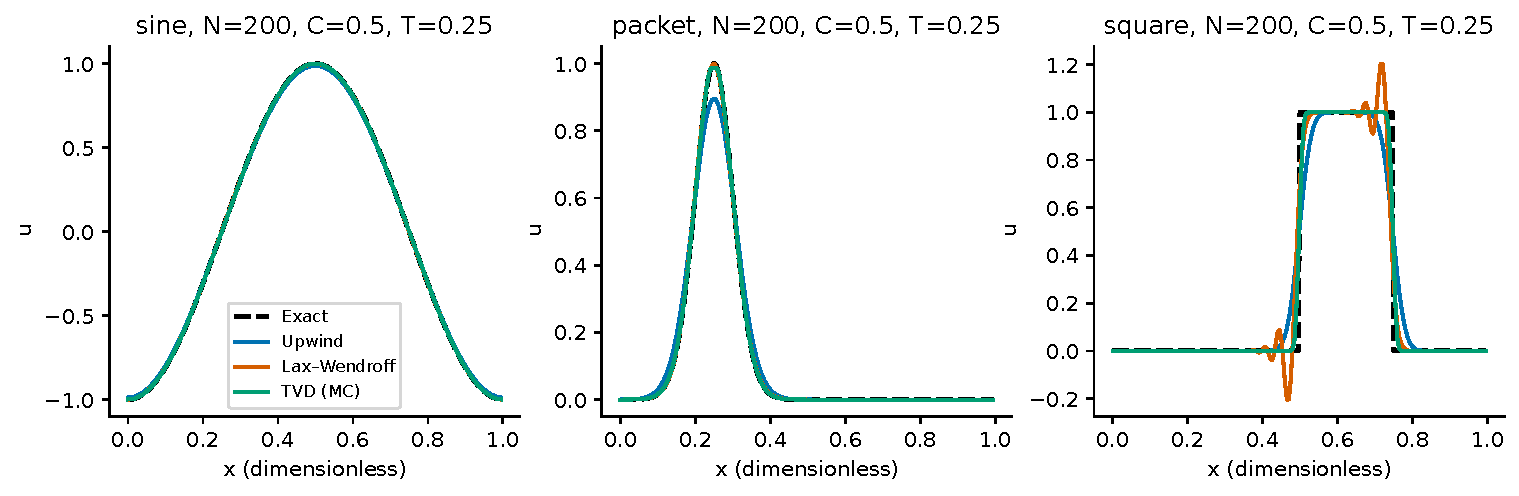
\includegraphics[width=.84\linewidth]{../results/figures/profiles.pdf}\par\vspace{1mm}\begin{block}{Takeaway}\small Sharper smooth profiles and bounded discontinuous profiles require different numerical compromises.\end{block}
\end{frame}
\begin{frame}{Dangerous-mode growth is distinct from ripples}
\centering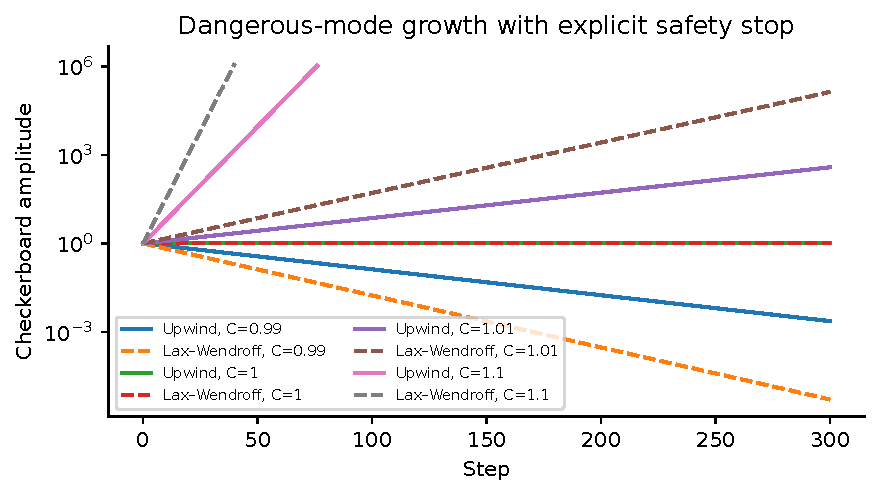
\includegraphics[width=.72\linewidth]{../results/figures/stability_growth.pdf}\par\vspace{1mm}\begin{block}{Takeaway}\small CFL violations amplify the dangerous mode. Stable jump ripples require a separate fidelity diagnosis.\end{block}
\end{frame}
\begin{frame}{Measured amplitude and numerical phase speed}
\centering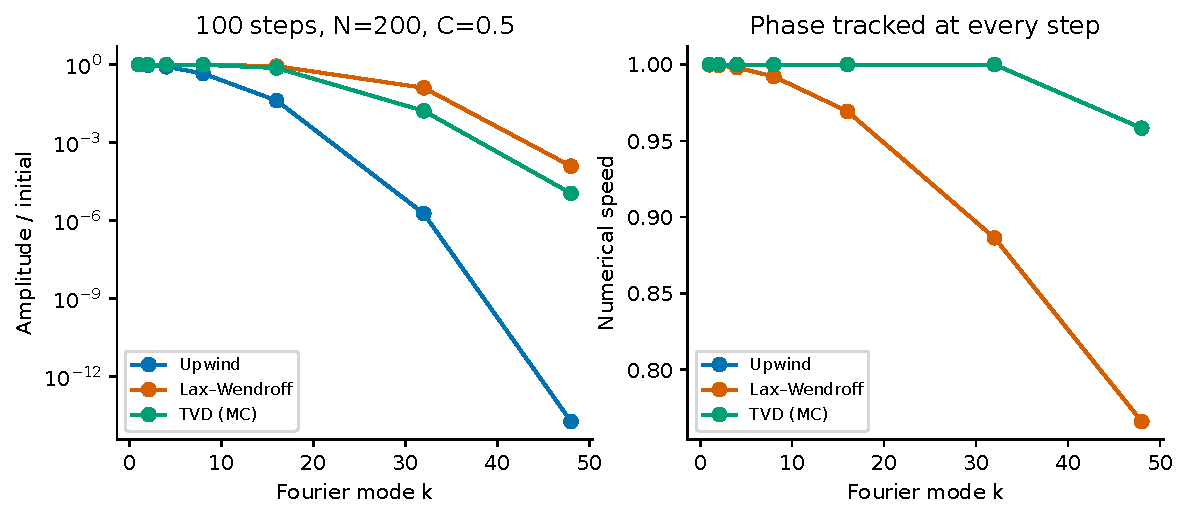
\includegraphics[width=.78\linewidth]{../results/figures/modal_fidelity.pdf}\par\vspace{1mm}\begin{block}{Takeaway}\small At C=0.5, upwind can retain phase while losing amplitude.\end{block}
\end{frame}
\begin{frame}{Errors accumulated over ten periods}
\centering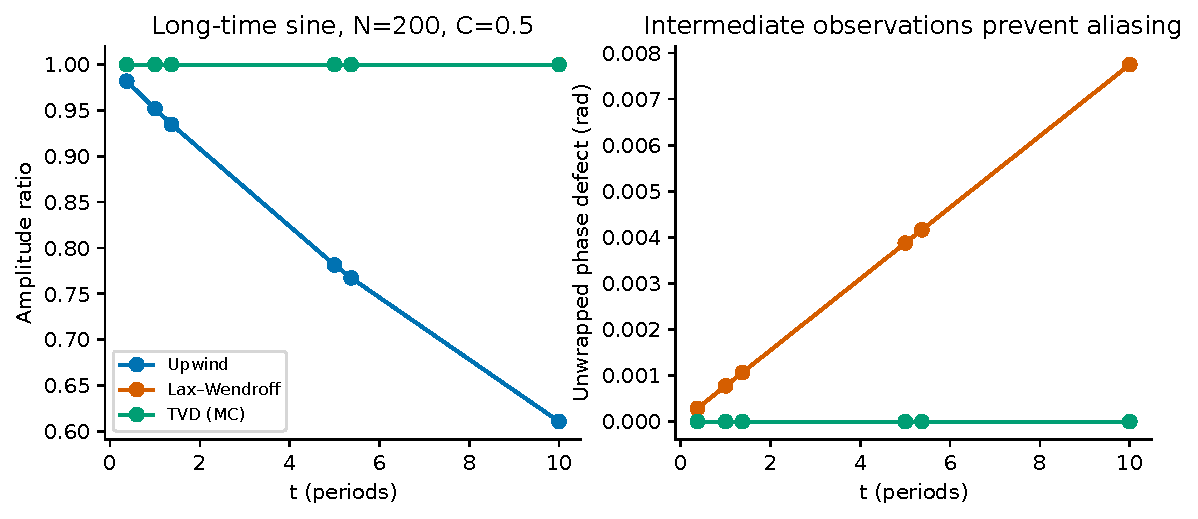
\includegraphics[width=.78\linewidth]{../results/figures/long_time.pdf}\par\vspace{1mm}\begin{block}{Takeaway}\small Mass can remain conserved while amplitude and phase errors accumulate.\end{block}
\end{frame}
\begin{frame}{Mass conservation and total variation}
\centering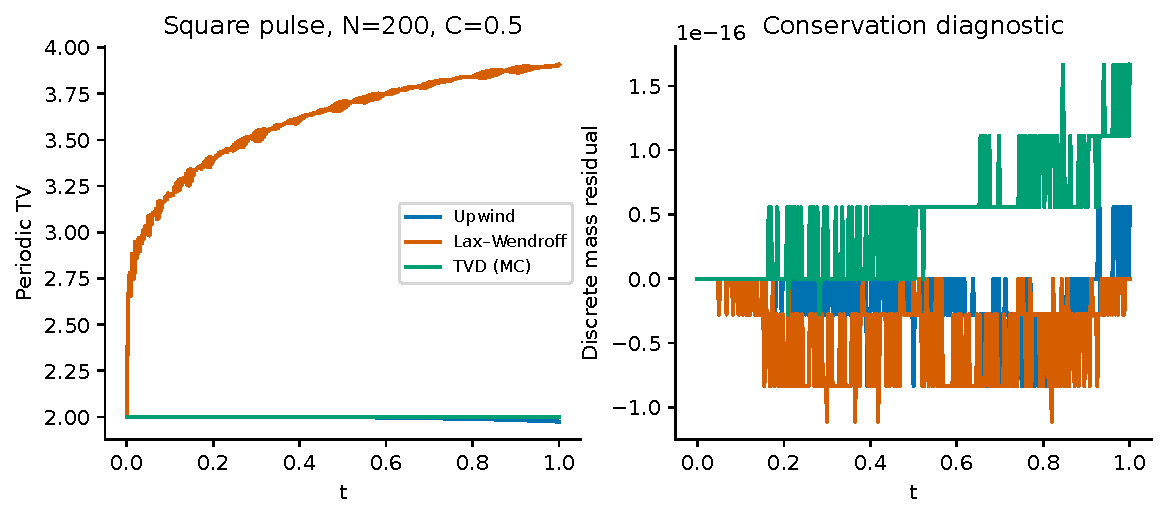
\includegraphics[width=.78\linewidth]{../results/figures/mass_tv.pdf}\par\vspace{1mm}\begin{block}{Takeaway}\small All methods conserve mass. Their total variation histories distinguish their behavior.\end{block}
\end{frame}
\begin{frame}{Cost at predeclared accuracy targets}
\centering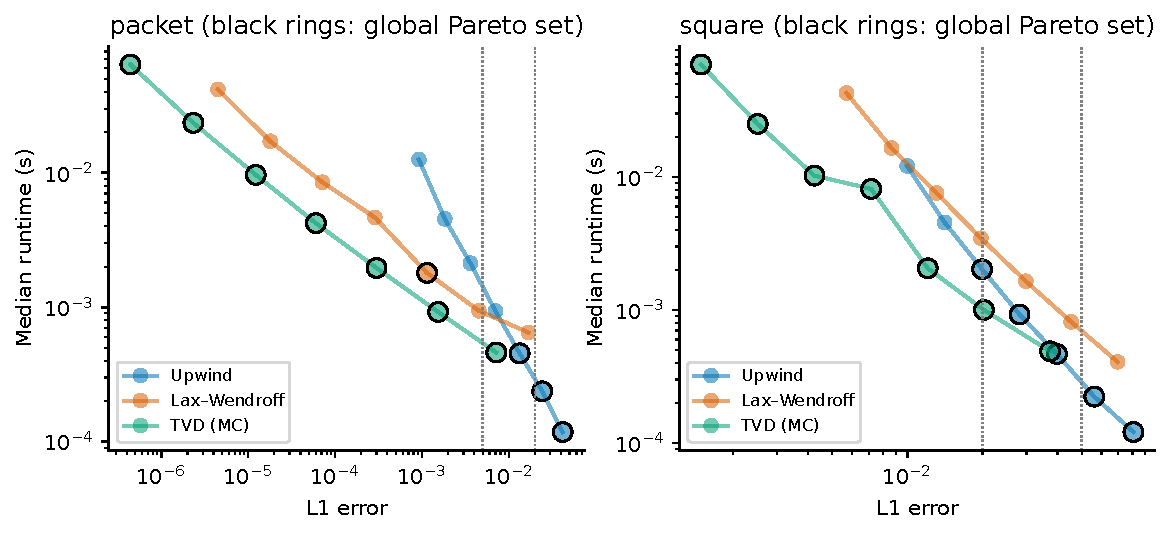
\includegraphics[width=.78\linewidth]{../results/figures/cost_accuracy.pdf}\par\vspace{1mm}\begin{block}{Takeaway}\small Compare the cost of meeting the same error target. The best tested choice depends on the datum.\end{block}
\end{frame}
\begin{frame}{Limitations and conclusion}
\begin{itemize}\item Scope: one-dimensional constant-speed periodic transport\item Nonlinear references have empirical tolerance checks\item Limiter extrema reduce accuracy and alter harmonics\item Timing rankings depend on hardware and short-run variability\item Student ICS, peer review and clean-room rerun remain pending\end{itemize}\vspace{4mm}\textbf{Conclusion:} Scheme choice depends on the datum, error target and fidelity constraints. TVD supplies a variation bound, not a universal error advantage.
\end{frame}\end{document}
